%

\documentclass[11pt]{article}
\usepackage[ruled,vlined]{algorithm2e}
\usepackage{amssymb}
\usepackage{amstext}
\usepackage{graphicx}
\usepackage{amsmath}
\usepackage{hyperref}
\graphicspath{{../images/}}
\newcommand{\fig}[1]{[Figure~(#1)]}
\begin{document}

%+Title
\title{Computing exact integrals of interpolated images within polygons and their derivatives}
\author{Martin de La Gorce}
\date{\today}
\maketitle
%-Title

%+Abstract
\begin{abstract}
   This document describes a numerical method to compute exactly the integral on an interpolated image inside a polygon and the derivatives of this integral with respect to the polygon's vertices locations. The text and formulas are mostly from my PhD Thesis \cite{DeLaGorce2009}
\end{abstract}
%-Abstract

%+Contents
%\tableofcontents
%-Contents

\section{Analytic formulas}

\subsection{Integal formulation}
Suppose we are given  
\begin{itemize}
\item a discretized function $f$ with domain $D=\{0,W-1\}\times\{0,H-1\}\subset \mathbb{R}^2$ taking values in $\mathbb R$. 
We formulate the interpolation of $f$ in the continuous domain $[0,W]\times[0,H]$ as a convolution by a kernel $k$:
\begin{equation}
f_c(x,y)=\sum_{(i,j)\in D} f(i,j) ~k(x-i,y-j)
\end{equation}

\item a non self-intersecting polygon defined through a sequence of $N$ vertices $$V=(v_1,\dots,v_N)$$ with $v_i=(x_i,y_i)$ circulating the polygon boundary counter-clockwise.
\end{itemize}
We denote $P(V)\subset \mathbb{R}^2$ the inside of the polygon and $\chi_P$ its characteristic function i.e. the function that takes value $1$ inside the plygon and $0$ ouside.

 The integral of the function $f_c$ inside the polygon $P(V)$ writes:
\
\begin{equation}
S(V)=\iint_{P(V)}f_c(x,y)dxdy
\label{eqn:integralef}
\end{equation}

\subsection{interpolation kernels}

The kernel depends on the type of interpolation we use:
\begin{itemize}
\item {The nearest neighbor} (shifted by 0.5) interpolation is obtained using the kernel that is constant and equal to 1 within the square $[0,1]^2$ and zeros outside the square:
\begin{equation}
k_{n}(x,y)=1\text{ if }(x,y)\in[0,1]^2,~0\text{ else}
\label{eqn:shifted_nearest_neighbor_kernel}
\end{equation}
Some basic variables manipulation will lead to: 
\begin{equation}
f_c(x,y)=\sum_{(i,j)\in L_d} f(i,j) k_{n}(x-i,y-j)=f(\left\lfloor x\right\rfloor,\left\lfloor y\right\rfloor)
\label{eqn:shifted_nearest_neighbor}
\end{equation}
with $\left\lfloor x\right\rfloor$ the greatest integer that is smaller or equal to $x$.
\item{The bilinear interpolation} is obtained using the kernel $k_b$ defined as follows:
\begin{equation}k_b(x,y)=(1-|x|)(1-|y|)\text{ if } (x,y)\in [-1,1]^2,~0 \text{ else}
\label{eqn:bilinear_kernel}
\end{equation}
\begin{figure}[t]
\begin{center}
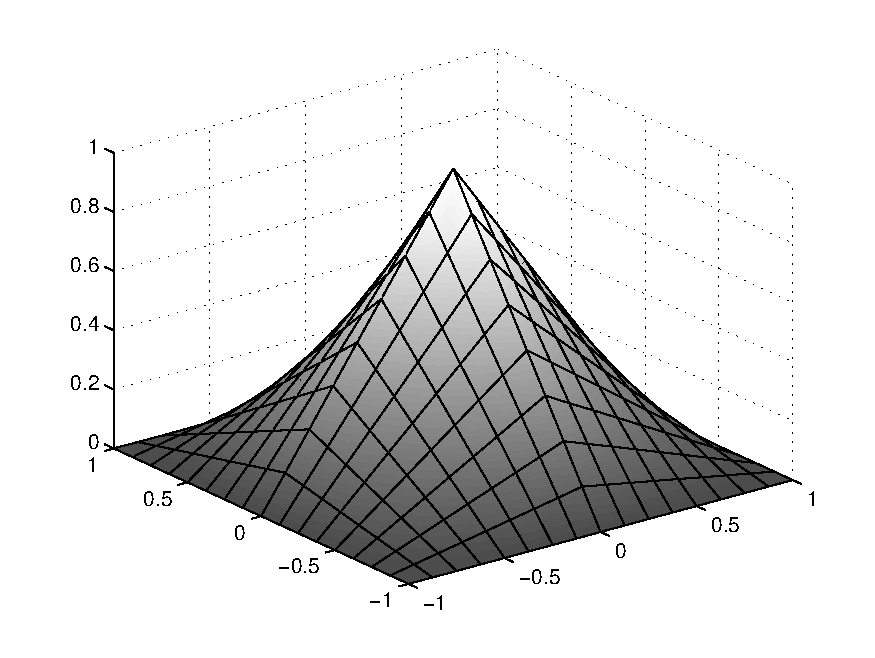
\includegraphics[width=4cm]{bilinear_kernel.pdf}
\caption[]{kernel for bilinear interpolation}
\label{fig:bilinear_kernel}
\end{center}
\end{figure} 


The kernel $k_b$ is shown in \fig{\ref{fig:bilinear_kernel}}. We define the function $\epsilon(x)=x-\lfloor x \rfloor$. With some rewriting we get: 
\begin{equation}
\begin{split}
f_c(x,y)=&(1-\epsilon(x))(1-\epsilon(y))f(\left\lfloor x\right\rfloor,\left\lfloor y\right\rfloor)\\&+
(\epsilon(x))(1-\epsilon(y))f(\left\lfloor x\right\rfloor+1,\left\lfloor y\right\rfloor)\\&+
(1-\epsilon(x))(\epsilon(y))f(\left\lfloor x\right\rfloor,\left\lfloor y\right\rfloor+1)\\&+
(\epsilon(x))(\epsilon(y))f(\left\lfloor x\right\rfloor+1,\left\lfloor y\right\rfloor+1)
\end{split}
\label{eqn:bilinear_interpolation}
\end{equation}
\end{itemize}








       
\subsection{First order derivates with respect to vertices}

\label{sec:silhouette_forces}

We aime at computing ${\partial S(V)}/{\partial v_j}$. Given a vertex of the polygon $v_k$ we use $v_{k-1}$ and $v_{k+1}$ to denote the preceding and following vertices in the polygon
The derivative of the functional $S(V)$ with respect to a vertex $v_k$ of the polygon writes :
        
\begin{equation}
\begin{split}
\frac{\partial S}{\partial v_k}=&J(v_k-v_{k-1})\int_0^1 f_c(tv_k+(1-t)v_{k-1})tdt\\
&+J(v_{k+1}-v_{k})\int_0^1 f_c(tv_{k}+(1-t)v_{k+1})tdt
\end{split}
\label{eqn:active_polygon}
\end{equation}
with $J$ the roation matrix defined by $$J=\left[^{~0}_{-1}~^{1}_{0}\right]$$
Let us introduce $l_k$ and $\hat{n}_k$ being the length and the normal of the segment $\overline{v_{k-1}v_k} $. We have: 
\begin{equation}
J(v_k-v_{k-1})=\hat{n}_k l_k
\end{equation}
One should point out that, for each vertex $v_k$, the information of the functional $f_c$ is being integrated along its adjacent edges. Using a mechanical metaphor, the resulting vector ${\partial S}/{\partial v_k}$ can be interpreted as a 2D data force acting on the polygon vertex $v_k$. 




 
 Note that $f_c$ does not have to be continuous everywhere for the integral  $S(P)$ to be differentiable. When using shifted-nearest-neighbor interpolation, $f_c$ is discontinuous for any point that lies on a vertical or an horizontal line of the pixel grid. However the first order derivative $\frac{\partial S}{\partial v_k}$ of the integral $S(V)$ is defined and continuous as long as none of the two adjacent polygon edge matches a vertical line or an horizontal line of the pixel grid.
 
 







\subsection{Second order derivatives}
\label{sec:second_order_derivatives}

In scenerios where we use the integral $S(V)$ as function we aim to minimize we may want to get access to the hessian of $S(V)$ in oder to be able to use a newton method. 

        The second order derivatives of the functional $S(V)$ with respect to two vertices of the polygon is derived by differentiating the equation eqn.\ref{eqn:active_polygon}. For any pair of vertices $(v_i,v_j)$ of the polygon the   order derivative ${\partial^2 S}/{\partial v_iv_j}$ is a 2 by 2 matrix. If the two vertices are not connected by an edge then ${\partial^2 S}/{\partial v_iv_j}= 0_{2\times2}$. As a consequence, if we gather all the derivatives $\frac{\partial^2 S}{\partial^2 v_j}$ into a single matrix $M$ composed of $2\times2$ sub-matrices $M_{2i:2i+1,2j:2j+1}$ corresponding to the $2\times 2$ matrices ${\partial^2 S}/{\partial v_iv_j}$, then this matrix $M$ is expected to be sparse and symmetric.

If two vertices are connected ($i=j+1$), then by setting $k=j$ in the equation eqn.\ref{eqn:active_polygon} and differentiating, we obtain: 
\begin{equation}
\begin{split}
\frac{\partial^2 S}{\partial v_{j+1}\partial v_j}=
&+J\int_0^1 f_c((1-t)v_{j+1}+tv_{j})tdt\\
&+J(v_{j+1}-v_{j})\int_0^1 \nabla f_c((1-t)v_{j+1}+tv_{j})(1-t)tdt
\end{split}
\label{eqn:second_order_derivative_qj_plus_one_qj}
\end{equation}
Because of the symmetry of derivatives we also get $\frac{\partial^2 S}{\partial v_{j}\partial v_{j+1}}=\frac{\partial^2 S}{\partial v_{j+1}\partial v_j}^T$. Note that the function $f_c$ should be differentiable almost everywhere along the two adjacent edges in order to have the second order derivative being properly defined. One should recall the bilinear interpolation $f_c$ is not differentiable for any point that lies on a vertical or an horizontal line of the pixel grid. Therefore the second order derivative ${\partial^2 S}/{\partial v_{j+1}\partial v_j}$  is defined for the bilinear interpolation if and only if the  edge $\overline{v_j v_{j+1}}$ does not match a vertical or an horizontal line of the image grid.

The second order derivative when $i=j$ writes 

\begin{equation}
\begin{split}
\frac{\partial^2 S}{\partial^2 v_j}=&J\int_0^1 f_c((1-t)v_{j-1}+tv_j)tdt-J\int_0^1 f_c((1-t)v_{j+1}+tv_{j})tdt\\
&+J(v_j-v_{j-1})\int_0^1 \nabla f_c((1-t)v_{j-1}+tv_j)t^2dt\\
&+J(v_{j+1}-v_{j})\int_0^1 \nabla f_c((1-t)v_{j+1}+tv_{j})t^2dt
\end{split}
\label{eqn:second_order_derivative_qjqj}
\end{equation}
The symmetry of the $2\times 2$ matrix ${\partial^2 L}/{\partial^2 v_j}$ is not obvious when considering this equation but can be proved using integration by parts.
The second order derivative ${\partial^2 S}/{\partial^2 v_{j}}$  is defined for bilinear interpolation and if none of the two adjacent edge $\overline{v_{j-1}v_j}$ $\overline{v_j v_{j+1}}$  matches a vertical or an horizontal line of the  image grid.    


 
 Note that in the context of active contour, several authors \cite{Hintermuller2004a,Burger2003,Hintermuller2004b,Bar2009} proposed the use of second order derivatives to accelerate the convergence.
Their formulations are done for general continuous and differentiable curves, generally require G\^ateaux derivatives in the derivation and are implemented using level set methods. In our case we have an explicit formulation of the region boundary as a polygon and, as a consequence, the second order derivatives are simpler to obtain.
%

\section{Relationship with antialiasing}

There is a strong relationship between the problem of computing \emph{exactly} the integral $S(V)$ and performing exact anti-aliased image of the polygon. In the context of computer graphics and signal processing in general the aliasing problem appears when a signal with high frequencies (spacial frequencies for an image) is sampled at a frequency smaller than $f_e/2$ ($f_e$ being the highest frequencies with no negligible energy in the signal). In computer graphics this appears when rendering geometric primitives with sharp boundaries on a discrete pixel grid. The abrupt intensity discontinuities at the boundaries cause high amplitude spectral components at extremely high frequencies.
 In practice if one discretizes an image composed of object with sharp boundaries, this result in "jaggies" or stair-like artifacts. In real cameras the optics creates some low-pass filtering (blurring) and pixel have spacial extension, which removes the aliasing effect. 
 
 Three techniques are now commonly used to reduce aliasing: pre-filtering, uniform super-sampling, and stochastic sampling. Pre-filtering consists in filtering the image in order to remove high spatial frequencies before sampling at pixel rates. For each pixel, the combination of the filtering and sampling operations can be interpreted as the computation of the scalar product of the filter kernel centered at the pixel with the continuous image.  
 The super-sampling methods consist in increasing the sampling rates (and hence the Nyquist rates) to some small multiple of pixel rates and then form each pixel intensity of the discrete image from a weighted average of neighboring samples. The super-sampling methods do not remove the discontinuous intensity changes, but reduce their magnitude, when the objects being drawn move continuously. Stochastic super-sampling methods randomly displace the super-sampling positions so that any aliased components appear as uncorrelated noise in the discrete image. 
 %This method can also be interpreted as approximated pre-filtering method, where the scalar product of the filter kernel centered at the pixel with the continuous image is approximated by a Monte-Carlo integration. 
 The noise induces temporal discontinuities in the discrete image when the objects being drawn displace continuously. Only the pre-filtering method can provide a discrete image that varies continuously when the rendered object displace continuously. 
 
 When the filter is the characteristic function of a unit square and the object being drawn are polygons with uniform colors, the antialiasing process can be re-interpreted as follows: 
Each polygon is clipped to the extend of the pixel and the contribution of each polygon to the pixel is weighted by area of the clipped region. This method is referred as the unweighted area sampling in \cite{Foley1996}(p133-134) and exact algorithms have been proposed in \cite{Catmull1978} and \cite{Duff1989} to compute the weights. In \cite{Catmull1978}, each polygon is clipped to each pixel using the Weiler-Atherton method which is quite expensive. In \cite{Duff1989} the approach is extended by replacing the area computation with a contour integral. Several optimizations that exploit the coherence of scan-conversion are also proposed. 
A method to compute exact antialiased triangles with any \emph{prisme spline} filter (which include the 2D box filter and the filter $k_b$ that is used for bilinear interpolation) has been proposed in \cite{McCool1995}.
Recent methods have been proposed to compute exact prefiltered antialiasing of polygon and bezier curves using various kernels \cite{Auzinger2015,Manson2013}.
In order to see the relationship between the problem of computing the integral $S(P)$ and performing anti aliasing we rewrite the integral defining $S(P)$ as follows:

\begin{equation}
\begin{split}
S(P)&=\iint f_c(x,y)\chi_P(x,y) dxdy\\
&=\iint \left[\sum_{(i,j)} f(i,j) k(x-i,y-j))\right]\chi_P(x,y)  dxdy\\
&=\sum_{(i,j)}  f(i,j) \underbrace{\iint  k(x-i,y-i))\chi_P(x,y)  dxdy}_{\tilde{M}(i,j)}
\end{split}
\label{eqn:antialiased_mask}
\end{equation}
The integral $S(V)$ is rewritten as a finite sum over the image pixels where the contribution of each pixel is weighted by $\tilde{M}(i,j)$.
The image $\tilde{M}$ can be interpreted as an anti-aliased version of the polygon binary image $M$ that is the pixel sampling of the characteristic function $\chi_P(x,y)$. Indeed $\tilde{M}(i,j)$ corresponds to the evaluation at the integer location $(i,j)$ of $\chi_P$ convolved with the kernel $k$. This convolution filters out (or reduce) high spatial frequencies. 


If we use the nearest neighbor interpolation shifted by 0.5 (eqn.\ref{eqn:shifted_nearest_neighbor}) one can easily interpret $\tilde{M}$ as the antialiased version to the polygon characteristic function $\chi_P$ using the \emph{unweighted area sampling} method. We rewrite the equation using the corresponding kernel $k$:
\begin{equation}
\begin{split}
\tilde{M}(i,j)&=\iint  k(x-i,y-j)\chi_P(x,y)  dxdy\\
&=\iint_{(x,y)_\in[i,i+1]\times[j,j+1]} \chi_P(x,y)dxdy\\
&=\iint_{\chi_P\cap[i,i+1]\times[j,j+1]} 1 dxdy
\end{split}
\end{equation}

For each pixel $(i,j)$ the value $\tilde{M}(i,j)$ is the measure of the area of intersection of the polygon $P(V)$ with the pixel $(i,j)$ that is spatially extended into a unit square $[i,i+1]\times[j,j+1]$. 
The integral $S(V)$ is a finite sum over the image pixels where the contribution of each pixel is weighted according to the surface of the intersection between the pixel and the polygon.

In order to compute the integral $S(V)$ we could use the antialiasing algorithms proposed in \cite{Catmull1978} and in \cite{Duff1989}. However, as shown in the next section, it is not actually needed to compute the antialiased image $M$ when computing $S(P)$. Our method uses the Green theorem to reduce the computation complexity by replacing the integral within the polygon interior by an integral along it boundary.

    
\section{Numerical integration} 

\subsection{using green's theorem}

The integral $S(V)$ of $f_c$ inside the polygon $P(V)$ can be rewritten as an integral on its boundary $\Gamma(V)\equiv \partial P(V)$ using the green's theorem:
 \begin{equation}
 \iint_{P(V)} f_c(x,y)dxdy=\oint_{\Gamma(V)}<F(s), \hat{n}(s)>ds
 \end{equation}
where $\hat{n}$ denotes the outward unit normal to $\Gamma(V)$, $ds$ the Euclidean arc length element and the circle in the right-hand integral indicates that the curve is closed and $F(s)$ is any function such that 
$div(F)=f_c$ 
 We choose  $F_y=0$ and  
 \begin{equation}F_x(x,y)=\int_{t=0}^x f_c(t, y)dt
 \label{eqn:Fx_definition}
 \end{equation} We have $F(s)=F_x(s).\hat{x}$. 
Using this function integral $S(V)$ becomes:

 \begin{equation}
 S(V)=\iint_{P(V)} f_c(x,y)dxdy=\oint_{\Gamma(V)} F_x(s) <\hat{n}(s).\vec{x}>ds
  \label{eqn:matching_cost_green}
 \end{equation}
The integral over $P(V)$ is reduced to an integral over the polygon boundary  $\Gamma(V)$.
If we use the shifted nearest neighbor interpolation then $F_x$ can be rewritten as:  
 \begin{equation}
F_x(x,y)=\sum_{u=0}^{\left\lfloor x\right\rfloor-1}f(u,\left\lfloor y\right\rfloor)+(x-\left\lfloor x\right\rfloor)f(\left\lfloor x\right\rfloor,\left\lfloor y\right\rfloor)
\label{eqn:FuNearestNeighbor}
\end{equation} 

\subsection{Line segments}
%
%
%

Let consider a segment $\overline{v_k v_{k+1}}$ whose extremities are $v_k\equiv(x_k,y_k)$ and $v_{k+1}\equiv(x_{k+1},y_{k+1})$ (like the segment $\overline{ab}$ in \fig{\ref{fig:trapezoid_integrals}.a}) The contribution of the segment $\overline{v_k v_{k+1}}$ to the integral is:
\begin{equation} 
C_k\equiv \int_{\overline{v_k v_{k+1}}} F_x(s)<\hat{x},\hat{n_k}> ds
\end{equation}

The normal vector of the segment $\hat{n_k}$ writes $\hat{n_k}=J{(v_{k+1}-v_{k})}/{l_k}$ with  $J=\left[^{~0}_{-1}~^{1}_{0}\right]$ and $l_k\equiv |v_k-v_{k+1}|$ the length of the segment.

$$<\hat{x},\hat{n_k}>=(y_{k+1}-y_k)/{l_k}$$

We can parameterize each segment linearly using a parameter $t\in[0,1]$: 
\begin{equation}
\overline{v_k v_{k+1}}=\{(1-t)v_k+tv_{k+1} ~|~ t\in[0,1]\}
\end{equation}
Using this parameterization for each segment, the integral rewrites:
\begin{equation} 
 C_k=(y_{k+1}-y_k) \int_0^1 F_x((1-t)v_k+t v_{k+1}) dt
 \label{eqn:ck_compact}
 \end{equation}

Supposing $y_k<y_{k+1}$, the segment can also be parameterized using the following curve
\begin{equation} 
r: 
\begin{array}{ccl}
[y_{k},y_{k+1}]&\rightarrow &{\mathbb R}^2\\
v &\mapsto & (\alpha v+\beta,v)
\end{array}
\end{equation}
with $\alpha=(x_k-x_{k+1})/(y_{k}-y_{k+1})$ and $\beta=x_{k}-\alpha y_k$. 
We get $\overline{v_{k}v_{k+1}}=r([y_k,y_{k+1}])$.
Using this parameterization of the segment, its contribution rewrites: 
\begin{equation} 
C_k=\int_{v=y_k}^{y_{k+1}} F_x(r(v))<\hat{n}_k,\vec{x}>|r'(v)|dv\\
\end{equation}


\begin{figure}[ht!]
\begin{center}
\begin{tabular}{ccc}
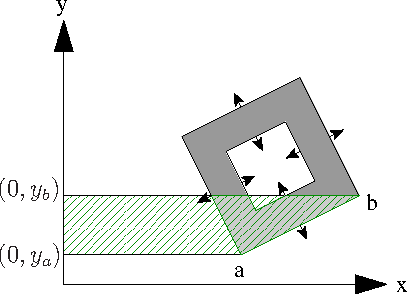
\includegraphics[height=2.5cm]{trapezoid_integrals_ab.pdf}&
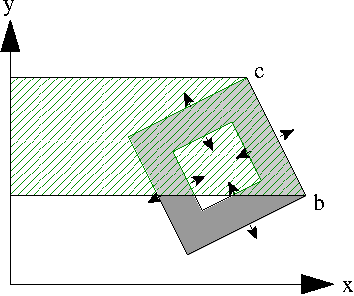
\includegraphics[height=2.5cm]{trapezoid_integrals_bc.pdf}&
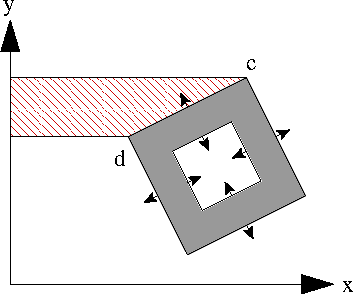
\includegraphics[height=2.5cm]{trapezoid_integrals_cd.pdf}\\
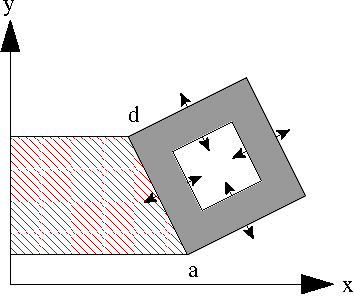
\includegraphics[height=2.5cm]{trapezoid_integrals_da.pdf}&
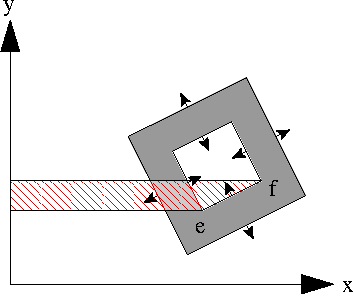
\includegraphics[height=2.5cm]{trapezoid_integrals_ef.pdf}&
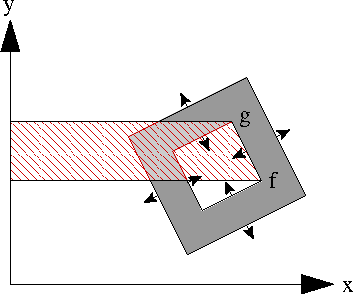
\includegraphics[height=2.5cm]{trapezoid_integrals_fg.pdf}\\
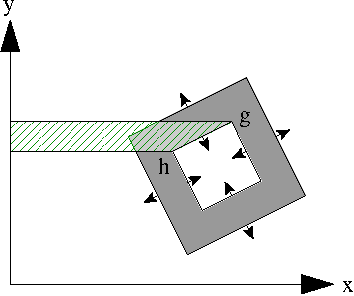
\includegraphics[height=2.5cm]{trapezoid_integrals_gh.pdf}&
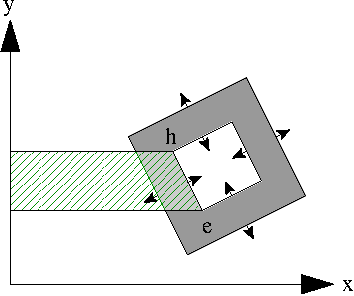
\includegraphics[height=2.5cm]{trapezoid_integrals_he.pdf}&
\end{tabular}
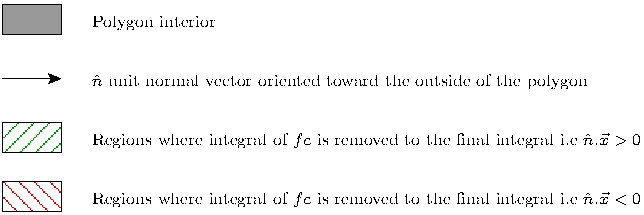
\includegraphics[width=11cm]{trapezoid_integrals_legend.pdf}
\caption[]{trapezoid integrals}
\label{fig:trapezoid_integrals}
\end{center}
\end{figure} 

Assuming that we are walking counterclockwise around the polygon, the outside normal $\hat{n}$ points towards the right while going from $v_k$ to $v_{k+1}$ (i.e. the inside of the polygon is on the left when going from $v_k$ to $v_{k+1}$). Because $y_k<y_{k+1}$ one can show that the outside normal points toward the right and  we have $<\hat{n}_k,\vec{x}>$ positive. With some calculus one can show that we have $<\hat{n}_k,\vec{x}>|r'(v)|=1$ and we get: 
\begin{equation} 
\begin{split}
C_k&=\int_{v=y_k}^{y_{k+1}} F_x(r(v))dv\\
&=\int_{v=y_{k}}^{y_{k+1}} F_x(\alpha v+\beta,u)du\\
&=\int_{v=y_{k}}^{y_{k+1}} \int_{u=0}^{\alpha v+\beta} f_c(u,v)du dv
\end{split}
\end{equation}

The last equation allows us to re-interpret easily the contribution of the segment to the contour integral. It corresponds to the integral of $f_c$ in the trapezoidal region on the left of the segment \fig{\ref{fig:trapezoid_integrals}} i.e with corners of coordinates $(x_{k},y_{k})$,$(x_{k+1},y_{k+1})$,$(0,y_{k+1})$, and $(0,y_{k})$. If the edge is on a hole boundary, the contribution of the segment to the contour integral is the integral of $-f_c$ in the trapezoidal region on the left of the segment.

 Depending on the interpolation scheme (shifted-nearest neighbor or bilinear) the function $f_c$ is either constant or quadric on each pixel. In order to compute exactly the integral of $F_x$ along the segment $\overline{v_k v_{k+1}}$ one needs to split this line segment into sub-pixel fragments. An example of such a fragmentation in shown in \fig{\ref{fig:fragment_segment}}. Each subpixel fragment is contained in an unit square pixel $[x,x+1]\times[y,y+1]$, with $(x,y)\in D$.  This is done by clipping the segment against each pixel, which can be done efficiently using the algorithm whose pseudo code is provided in \ref{alg:clipSegmentOnPixelGrid}. The segment  $\overline{v_k v_{k+1}}$ is clipped by computing its intersections with the pixel grid that is composed of vertical lines with integer $x$ coordinates and horizontal lines with integer $y$ coordinates. The intersections are detected in an order such that their distance from $v_k$ is increasing. Each segment whose extremities are two successive intersections with the pixel grid is contained in a pixel square.

\begin{figure}[ht]
\begin{center}
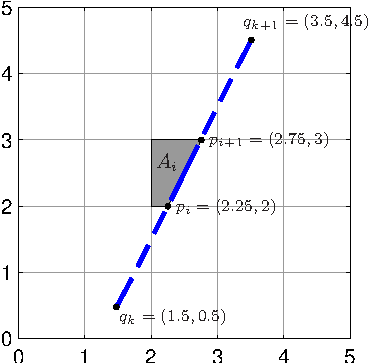
\includegraphics[height=5cm]{fragment_segment_1.pdf}
\caption[]{Sub-pixel fragmentation of a segment. Example with $v_k=(1.5,0)$ and $v_{k+1}=(3.5,4.5)$}
\label{fig:fragment_segment}
\end{center}
\end{figure} 



Once the segment is partitioned into sub-pixel fragments we can easily perform integration on each fragment.
Let $p_i\equiv(x_i,y_i)$ and $p_{i+1}\equiv(x_{i+1},y_{i+1})$ be the extremities of a subpixel segment of $\overline{v_k v_{k+1}}$. We have $\overline{p_i p_{i+1}}\subset \overline{v_kv_{k+1}}$. The two extremities $p_i$ and $p_{i+1}$ belong to the same pixel which means that we have 
\begin{equation}
\left\{
\begin{array}{lcl}
(x_i,y_i) &\in& [k,k+1]\times [l,l+1]\\  
(x_{i+1},y_{i+1})& \in &[k,k+1]\times [l,l+1]
\end{array}
\right.
\end{equation}
with $k=\lfloor(x_i+x_{i+1})/2\rfloor$ and $l=\lfloor(y_i+y_{i+1})/2\rfloor$.
Note that we may have $\left\lceil x_i\right\rceil\neq\left\lceil x_{i+1}\right\rceil$ of $\left\lceil y_i\right\rceil \neq \left\lceil y_{i+1}\right\rceil$ if $x_i$ or $y_i$ are integers.
We denote $c^i\equiv(x_c^i,y_{ci})$ the center of the $i^{th}$ subpixel segment. we have $x_{ci}=(x_i+x_{i+1})/2$ and   $y_{ci}=(y_i+y_{i+1})/2$. We introduce the two variables $\Delta_{yi} \equiv y_{i+1}-y_{i}$ and $\Delta_{xi} \equiv x_{i+1}-x_{i}$. 

\subsubsection{Nearest neighbor interpolation}
\label{sec:nn_interpolated2Dintegral}

If we use the shifted nearest neighbor interpolation with the kernel $k_n$, then the function $f_c$ is constant within each unit square corresponding to a pixel. Furthermore, the function $F_x$ is linear within each of these squares.
Because $p_i$ and $p_i+1$ belong to the same pixel and we use the shifted nearest neighbor interpolation, the function $u\mapsto F_x(r(u))$ is linear on the interval $[y_i,y_{i+1}]$ and we can evaluate the integral by simply evaluating  the center point $c^i$ of the interval:

\begin{equation} 
\begin{split}
C_i&=(y_{i+1}-y_i)F_x\big(r((y_i+y_{i+1})/2)\big)\\&=
\Delta_{yi} F_x(x_{ci},y_{ci})
\end{split}
\end{equation}

We get from eqn \ref{eqn:FuNearestNeighbor}: 

\begin{equation} 
C_i=(y_{i+1}-y_i)\sum_{u=0}^{\left\lfloor x_c\right\rfloor-1}f(u,\left\lfloor y_c\right\rfloor)+\underbrace{(y_{i+1}-y_i)(x_c-\left\lfloor x_c\right\rfloor)}_{A_i}f(\left\lfloor x_c\right\rfloor,\left\lfloor y_c\right\rfloor)
\end{equation}

The value of $A_i$ is the area of the intersection of the trapezoidal region on the left of the fragment $\overline{p_ip_{i+1}}$ and the pixel as shown in \fig{\ref{fig:fragment_segment}}.





Consequently, our algorithm could be easily adapted to implement the antialiasing method we referred as the ``unweighted area sampling'' in the previous section. After meticulous search of similar algorithm in the literature, it appeared that our method bears similarities with the one proposed in \cite{Cheng1992} that adapts the Bresenham \cite{Bresenham1965} line rasterization method using two error variables. However, our method that clips segment on pixel grids appears to be simpler. The source code can be found on the Graphic Gems Repository \footnote{\url{http://tog.acm.org/resources/GraphicsGems/gemsiii/edgeCalc.c}}. Our method also bears similarities with antialiasing methods proposed  in \cite{Pitteway1980} \footnote{A pseudo code can be found here \url{http://www710.univ-lyon1.fr/~jciehl/Public/educ/ENS/2003/antialiassage.pdf}},\cite{Wu1991} and \cite{Fujimoto1983}. These algorithms adapt the Bresenham \cite{Bresenham1965}  rasterization line algorithm to perform antialiasing. These algorithms differ from our contribution because they consists in clipping the line segment only against vertical lines of the pixel grid or only against horizontal lines, depending on the direction of the line segment. The resulting approximate coverage agrees with the exact coverage only when the edge does not cross a line on the pixel grid that is orthogonal to the set of lines chosen for the clipping. Furthermore these algorithms do not handle line ends properly. 

\subsubsection{Bilinear interpolation}

\label{sec:BilinearInterpolationIntegration}

From the equation eqn.\ref{eqn:bilinear_interpolation} that defines the bilinear interpolation and the equation eqn.\ref {eqn:Fx_definition} that defines $F_x$ we get:
    
\begin{equation} 
\begin{split}   
F_x(x,y)=&\epsilon(y) \left(\sum_{u=0}^{\lfloor x \rfloor}f(u,\lceil y \rceil)-\frac{1}{2} f(0,\lceil y \rceil)-\frac{1}{2}f(\lfloor x \rfloor,\lceil y \rceil)\right)\\
&+(1- \epsilon(y)) \left(\sum_{u=0}^{\lfloor x \rfloor}f(u,\lfloor y \rfloor)-\frac{1}{2} f(0,\lfloor y \rfloor)-\frac{1}{2}f(\lfloor x \rfloor,\lfloor y \rfloor)\right)\\
&+\epsilon(x)f_c(\lfloor x\rfloor+\frac{\epsilon(x)}{2},y)
\end{split}
\end{equation}     
    The contribution of the $i^{th}$ sub-pixel fragment can be shown to be:     
\begin{equation}  
\begin{split}
C_i=\Delta_{yi}  F_x(\lfloor x_{ci} \rfloor,y_{ci})
&+c_{00}f(\lfloor x_{ci} \rfloor,\lfloor y_{ci} \rfloor)
+c_{10}f(\lfloor x_{ci} \rfloor+1,\lfloor y_{ci} \rfloor)\\
&+c_{01}f(\lfloor x_{ci} \rfloor,\lfloor y_{ci} \rfloor+1)
+c_{11}f(\lfloor x_{ci} \rfloor+1,\lfloor y_{ci} \rfloor+1)
\end{split}
\end{equation}

with $c_{00}$,$c_{10}$,$c_{01}$ and $c_{11}$ defined as:        
\begin{eqnarray}        
c_{11} &\equiv&  \frac{\Delta_{xi}\Delta_{yi}^2}{12}   \epsilon(x_{ci}) +\frac{\Delta_{yi}\Delta_{xi}^2}{24}\epsilon(y_{ci})\\
c_{10} &\equiv& -c_{11}+\frac{\Delta_{yi}\Delta_{xi}^2}{24} \\
c_{01} &\equiv& -c_{11}+\frac{\Delta_{xi} \Delta_{yi}^2}{12}\\
c_{00} &\equiv& -c_{10}- \frac{\Delta_{xi} \Delta_{yi}^2}{12} 
\end{eqnarray}
             
These equations are quite tedious to derive and we used the Maple symbolic computation tool.
Note that  methods to integrate 2D polynomials into polygons have been proposed in \cite{Tumblin2006,Steger1996,Liggett1988,Singer1993,Strachan1990} and their result might be useful to extend the integration in the polygon for other polynomial interpolation schemes such as bi-cubic interpolation
The method proposed in \cite{McCool1995} to render antialiased triangles is also of interest.     
        
           




 \subsection{Derivatives}
 
 In order to compute the \emph{exact} derivative given by equation \ref{eqn:active_polygon}, we need to clip each segment onto the pixel grid and to integrate on each subpixel fragment. 
By stating that the gradient is \emph{exact} we mean that, given a definition of $f_c$ as nearest neighbor or bilinear interpolation of $f$, we are able to compute exactly the equation \ref{eqn:active_polygon}. The method to compute exactly the gradient is very similar to the method that is used to compute exactly the integral $S(V)$. The pseudo code for shifted nearest neighbor interpolation is at alg.\ref{alg:integrateSegmentDerivativeNearestNeighbor} and the pseudo code for the bilinear interpolation at alg.\ref{alg:integrateSegmentDerivativesBilinear} (this second algorithm also compute second order derivatives whose derivation is explained in the section \ref{sec:second_order_derivatives}).
    



The pseudo-code to compute first and second order derivative for bilinear interpolation of $f$ is provided in alg.\ref{alg:integrateSegmentDerivativesBilinear} 

Note that we could approximate the integrals in the gradient and the hessian by finite sums through uniform sampling of points along each segment and evaluation of $f_c$ and $\nabla f_c$ at these locations. However the equation \ref{eqn:second_order_derivative_qjqj} does not exhibit obvious symmetry and the approximate Hessian we would obtain is not symmetric. Therefore we would have to impose the symmetry of the Hessian by averaging the computed Hessian matrix and its transpose.

The Hessian we obtain using the exact integration along the edges using the algorithm alg.\ref{alg:integrateSegmentDerivativesBilinear} is symmetric up to round-off errors. 
\subsection{Improvements}
The symmetry of the hessian is not obvious from our  equations, maybe we could obtain an expression where the symmetry is obvious and hopefully that would lead to a slightly simplier expression that would require a bit less computation for its exact computation.

\newpage









\begin{algorithm}[h!]
%\linesnumbered
\caption{clipSegmentOnPixelGrid}
\label{alg:clipSegmentOnPixelGrid}
%\SetLine

\KwData{Two segment extremities $a\equiv(x_a,y_a)$ and $b\equiv(x_b,y_b)$ }
Result:{a list of Point $p_1,\dots,p_N$ and their normalized curvilinear  coordinate $t_1,\dots t_N\in[0,1]$ on the segment such that 
$p_1=(x_a,y_a)$, $p_N=(x_b,y_b)$, $\overline{ab}=\bigcup_{i=1}^N\overline{p_i,p_{i+1}}$ and for each $i$ the two segments extremities $p_i$ and $p_{i+1}$ lies inside the same pixel}


\tcp{\emph{get the first intersection with a vertical line}}
\eIf {$x_b>x_a$} 
{$\delta_v^x\leftarrow1$;~$x_v\leftarrow\left\lfloor x_a\right\rfloor+1$\;} 
{$\delta_v^x\leftarrow-1$;~$x_v\leftarrow\left\lceil x_a\right\rceil-1$\;}
\eIf {$\delta_x x_v<\delta_x x_b$}
{
$N_v\leftarrow \left\lceil \delta_x(x_b-x_v)\right\rceil$;~
$\delta_v^T\leftarrow \delta_v^x/(x_b-x_a)$;~$\delta_v^y\leftarrow (y_b-y_a)\delta_v^T$\;
$y_v\leftarrow \delta_v^x\delta_v^y (x_v-x_a)+y_a$;~
$t_v\leftarrow \delta_v^x\delta_v^T (x_v-x_a)$\;
}
{$N_v=0$;$t_v=1$\; }


\tcp{\emph{get the first intersection with an horizontal line}}
\eIf {$y_b>y_a$} 
{$\delta_h^y\leftarrow1$;~$y_h\leftarrow\left\lfloor y_a\right\rfloor+1$\;} 
{$\delta_h^y\leftarrow-1$;~$y_h\leftarrow\left\lceil y_a\right\rceil-1$\;}
\eIf {$\delta_y y_h<\delta_y y_b$}
{
$N_h\leftarrow \left\lceil \delta_y(y_b-y_h)\right\rceil$;~
$\delta_h^T\leftarrow \delta_h^y/(y_b-y_a)$;~
$\delta_h^x\leftarrow (x_b-x_a)\delta_h^T$\;
$x_h\leftarrow \delta_h^x\delta_h^y (y_h-y_a)+x_a$;~
$t_h\leftarrow \delta_v^y\delta_v^T (y_v-y_a)$\;
}
{$N_h \leftarrow  0$;$t_h=1$\;}

$p_1=(x_a,y_a)$;~$t_1=0$\;

\tcp{\emph{Loop until it reaches the extremity $b$}}
$N \leftarrow N_h+N_v+2$\;
\For{$k \leftarrow 2$ \KwTo $N$}
{
\eIf{$t_v<t_h$} 
{
\tcp{\emph{the next intersection is with a vertical line}}
$p_k\leftarrow (x_v,y_v)$;~$t_k\leftarrow t_v$\;
\tcp{\emph{get the next intersection with an vertical line}}
$(x_v,y_v,t_v)\leftarrow (x_v+\delta_v^x,y_v+\delta_v^y,t_v+\delta_v^T)$\;
}
{
\tcp{\emph{The next intersection is with an horizontal line}}
$p_k\leftarrow (x_h,y_h)$;~$t_k\leftarrow t_h$\;
\tcp{\emph{get the next intersection with an horizontal line}}
$(x_h,y_h,t_h)\leftarrow (x_h+\delta_h^x,y_h+\delta_h^y,t_h+\delta_h^T)$\;
}
}
$p_{N}\leftarrow (x_b,y_b)$;~$t_N=1$\;
\end{algorithm}


\clearpage

      

\begin{algorithm}[ht]
%\linesnumbered
\caption{integrateSegmentDerivativeNearestNeighbor}
\label{alg:integrateSegmentDerivativeNearestNeighbor}
%\SetLine

\KwData{The polygon vertices $(v_i)_{i=1}^N$ and a discretized function $f(x,y)$ }
\KwResult{The derivatives $\dot{v}_i \equiv \frac{\partial I}{\partial v_i}$ of the integral $I$ of $f_c$ inside the polygon with $f_c$ the shifted nearest neighbor interpolation of $f$  }


\For{$i \leftarrow 1$ \KwTo $N$}
{
$\dot{v}_i \leftarrow [0,0]^T$;
}

\tcp{\emph{loop over edges of the polygon}}

\For{$i \leftarrow 1$ \KwTo $N$}
{
$j=mod(i,N)+1$\;

\tcp{\emph{clip the segment $\overline{v_i,v_j}$ on the pixel grid}}
$(p_k,t_k)_{k=1}^K\leftarrow\text{intersectSegment}(v_i,v_j)$\;
\tcp{\emph{loop over subpixel fragments}}
\For{$k \leftarrow 1$ \KwTo $K-1$}
{
\tcp{\emph{compute the middle point of the subpixel fragment}}
$x_c=(x_k+x_{k+1})/2$\;
$y_c=(y_k+y_{k+1})/2$\;
$t_c=(t_k+t_{k+1})/2$\;
$\Delta_t=(t_{k+1}-t_{k})$\;
\tcp{\emph{add contribution of fragment to the derivative}}
$\dot{v}_i \leftarrow \dot{v}_i + \left[^0_1~^{-1}_{~0}\right](v_j-v_i)(t_{k+1}-t_{k})t_c f(\left\lfloor x_c\right\rfloor,\left\lfloor y_c\right\rfloor)$\;
$\dot{v}_j  \leftarrow \dot{v}_j + \left[^0_1~^{-1}_{~0}\right](v_j-v_i)(1-t_c)f(\left\lfloor x_c\right\rfloor,\left\lfloor y_c\right\rfloor)$\;
}
}
\end{algorithm}



      
      \clearpage
      
In order to make the pseudo-code \ref{alg:integrateSegmentDerivativesBilinear} comprehensive, we explain some of the intermediary variables: 
\begin{eqnarray}
x(t)&=& (1-t)x_i + tx_j=A_x[1,t]^T\nonumber\\
y(t)&=& (1-t)y_i + ty_j=A_x[1,t]^T\nonumber\\
x(t)y(t)&=&A_xy[1,t,t^2]^T \label{eqn:xtyt}
\end{eqnarray}
\begin{eqnarray}
v_d&=&\int_{t_{k}}^{t_{k+1}} t^{d-1} dt  \label{eqn:vd}
\end{eqnarray}
\begin{eqnarray}
c_0&=&\int_{t_k}^{t_{k+1}} t^{d-1} dt \nonumber\\
c_x&=&\int_{t_k}^{t_{k+1}} \epsilon(x(t))t^{d-1} dt\nonumber\\
c_y&=&\int_{t_k}^{t_{k+1}} \epsilon(y(t))t^{d-1} dt\nonumber\\
c_{xy}&=&\int_{t_k}^{t_{k+1}} \epsilon(x(t))\epsilon(y(t))t^{d-1} dt
\label{eqn:cxy}
\end{eqnarray}
 After summation over all subpixel fragments of a segment we have:
\begin{eqnarray}
\beta&=&\int_{0}^1  [1,t,t^2]^T f_c(x(t),y(t))) dt\nonumber\\
\gamma&=&\int_{0}^1 [1,t,t^2]^T \nabla fc(x(t),y(t))) dt
\label{eqn:beta_gamma}
\end{eqnarray}
And we finally obtain.
\begin{eqnarray}
\alpha_1&=&\int_0^1 f_c((1-t)v_i+t v_{j}) t dt\nonumber\\
\alpha_2&=&\int_0^1 f_c((1-t)v_i+t v_{j}) (1-t) dt\nonumber\\
\alpha_3&=&\int_0^1 \nabla { f_c}((1-t)v_i+t v_{j}) ~t^2 dt\nonumber\\
\alpha_4&=&\int_0^1 \nabla { f_c}((1-t)v_i+t v_{j}) (1-t)^2 dt\nonumber\\
\alpha_5&=&\int_0^1 \nabla { f_c}((1-t)v_i+t v_{j}) (1-t)~t ~dt
\label{eqn:alpha}
\end{eqnarray}
      \newpage
      
      
\begin{algorithm}[ht!]
%\linesnumbered
\caption{integrateSegmentDerivativesBilinear}
\label{alg:integrateSegmentDerivativesBilinear}
%\SetLine

\KwData{The polygon vertices $(v_i)_{i=1}^N$ and a discretized function $f(x,y)$ }
\KwResult{The derivatives $\dot{v}_i \equiv \frac{\partial I}{\partial v_i}$ and $H_{ij}\equiv  \frac{\partial^2 I}{\partial v_iv_j}$of the integral $I$ of $f_c$ inside the polygon with $f_c$ the bilinear interpolation of $f$ }


\tcp{\emph{loop over edges of the polygon}}

\For{$i \leftarrow 1$ \KwTo $N$}
{
 $j=mod(i,N)+1$\;

 $\beta \leftarrow 0_{3 \times 1}$;~
 $\gamma \leftarrow 0_{3 \times 2}$

$(p_k,t_k)_{k=1}^K\leftarrow\text{intersectSegment}(v_i,v_j)$;\tcp{\emph{clip the segment $\overline{v_i,v_j}$ on the pixel grid}}

\tcp{\emph{loop over subpixel fragments}}
\For{$k \leftarrow 1$ \KwTo $K-1$}
{
$x_c=(x_k+x_{k+1})/2$;~$y_c=(y_k+y_{k+1})/2$;~$t_c=(t_k+t_{k+1})/2$\;
$\Delta_x=x_{k+1}-x_{k}$;~$\Delta_y=y_{k+1}-y_{k}$;~$\Delta_t=t_{k+1}-t_{k}$\;
$A_x \leftarrow [\epsilon(x_c)-(\Delta_x t_c/\Delta_t),~\Delta_x/\Delta_t]$; \tcp{\emph{see eqn.\ref{eqn:xtyt}}}
$A_y \leftarrow [\epsilon(y_c)-(\Delta_y t_c/\Delta_t),~\Delta_y/\Delta_t]$\; 
$A_{xy}=[A_x(1)A_y(1),~A_x(1)A_y(2)+A_x(2)A_y(1),~A_x(2)A_y(2)]$;

\For{$d \leftarrow 1$ \KwTo $5$}
{    $v_d=((t_{k+1})^d-(t_{k})^d)/d$;~\tcp{\emph{see eqn.\ref{eqn:vd}}}
}
$f_{00}\leftarrow f(\left\lfloor x_c\right\rfloor,\left\lfloor y_c\right\rfloor)$;~
$f_{01}\leftarrow f(\left\lfloor x_c\right\rfloor,\left\lfloor y_c\right\rfloor+1)$\;
$f_{10}\leftarrow f(\left\lfloor x_c\right\rfloor+1,\left\lfloor y_c\right\rfloor)$;~
 $f_{11}\leftarrow f(\left\lfloor x_c\right\rfloor+1,\left\lfloor y_c\right\rfloor+1)$\;
 $b_0 \leftarrow f_{00}$;~  
 $b_x \leftarrow f_{10}-f_{00}$;~
 $b_y \leftarrow f_{01}-f_{00}$\;
 $b{xy} \leftarrow f_{11}-f_{10}+f_{00}-f_{01}$\;
 
\For{$d \leftarrow 1$ \KwTo $3$}
{
$c_0 \leftarrow v_d$\;$c_x \leftarrow A_x[v_d,v_{d+1}]^T$;~\tcp{\emph{see eqn.\ref{eqn:cxy}}}
$c_y \leftarrow A_y[v_d,v_{d+1}]^T$\;
$c_{xy} \leftarrow A_{xy}[v_d,v_{d+1},v_{d+2}]^T$\;
$\beta_d \leftarrow \beta_d + b_0 c_0+b_x c_x+b_y c_y+b_{xy}c_{xy}$;~\tcp{\emph{see eqn.\ref{eqn:beta_gamma}}}
$\gamma_{[d,:]} \leftarrow \gamma_{[d,:]}  +b_{xy}c_y + [b_x,b_y]^T c_0$\;
}
}
 $\alpha_1 \leftarrow [0,1,0] \beta$;~\tcp{\emph{see eqn.\ref{eqn:alpha}}}
 $\alpha_2 \leftarrow [1,-1,0]\beta $; 
 $\alpha_3 \leftarrow [0,0,1] \gamma$;
 $\alpha_4 \leftarrow [1,-2,1]\gamma$;
 $\alpha_5 \leftarrow [0,1,-1]\gamma$; 
$J\leftarrow \left[^0_1~^{-1}_{~0}\right]$\;  
$\dot{v}_j \leftarrow \dot{v}_j  + J(v_j-v_i) \alpha_1$\;
$\dot{v}_i \leftarrow  \dot{v}_i + J(v_j-v_i) \alpha_2$\;         
 $H_{ii} \leftarrow  H_{ii} -J \alpha_2+J (v_j-v_i) \alpha_4$\; 
 $H_{jj} \leftarrow  H_{jj} +J \alpha_1+J (v_j-v_i) \alpha_3$\;
 $H_{ji} \leftarrow J \alpha_2+J (v_j-v_i) \alpha_5$\;
 $H_{ji} \leftarrow H_{ji}^T$\;
}
\end{algorithm}
 
\newpage
\newpage

{\small
\bibliographystyle{plain}
\bibliography{biblio}
}

\end{document}


